\documentclass{sig-alternate}
	\usepackage{fourier}
	\usepackage{tikz}

	\usepackage{amsmath}
	\usepackage{amsfonts}
	\usepackage{amssymb}

	\usepackage{graphicx}

	\newcommand{\Fone}{$F_1$}
	\renewcommand{\vec}[1]{\mathbf{#1}}

	\newcommand{\argmin}{\operatornamewithlimits{argmin}}
	\newcommand{\argmax}{\operatornamewithlimits{argmax}}
\begin{document}
\sloppy

\title{Stack Exchange Tag Prediction through Keyword Extraction}
\numberofauthors{2}
\author{
	\alignauthor
	Gio Borje \\
	\affaddr{University of California, Irvine} \\
	\email{gborje@uci.edu}
	\alignauthor
	Paul Kang \\
	\affaddr{University of California, Irvine} \\
	\email{pdkang@uci.edu}
}
\maketitle

\begin{abstract}
	Stack Exchange is a set some of the most renown, community-driven
	question and answer sites. The annotation of questions with tags
	enables users to find and respond to questions of interest
	immediately. However, the annotation of questions with tags is tedious
	and error-prone because users may not be aware of the best tags to
	categorize their question. By automating the process of annotating
	questions with tags, the community is relieved of their crowdsourcing
	work and enables them to focus on the important aspect of asking and
	answering questions. We survey several approach to keyword extraction
	and tag suggestion to Stack Exchange posts using a Bag-of-Words (BOW)
	model and show that Support Vector Machines have the best accuracy.
\end{abstract}

\section{Introduction} % (fold)
\label{sec:Introduction}
	Kaggle is a community of data scientists focused on solving complex
	data-science problems by providing company-hosted, public, data
	science competitions. Competitions proceed as follows. A
	company begins hosting a competition by providing a public data set as
	well as an evaluation metric. Participants register for the
	competition, download the data set, manipulate the data, and creates
	an appropriate model. Then, the participants download the test data
	set and make predictions on the test data using the trained models.
	The predictions for the test data are uploaded into the competition
	page, scored by the specified evaluation metric, and ranked
	accordingly on a public leaderboard.

	This challenge is proposed through Kaggle: given only the title and body of
	a question, predict the question's tags. The training data set provided
	comes from Stack Exchange sites which mixes both technical and nontechnical
	questions. We do not solve this challenge. Instead, we survey a potential
	set of classifiers to see which classifier performs uniformly better than
	all others given the data set. Specifically, we evaluate a Bernoulli
	na\"{i}ve Bayes classifier, Linear Support Vector Machine, Random Forest
	classifier, and a Gradient Boosting Machine.

	The evaluation metric for this competition uses the Mean \Fone-Score
	which is commonly used to measure classification accuracy through
	\emph{precision} and \emph{recall}. Precision can be defined as the
	ratio of true positive classifications over the true and false
	positive classifications. The recall can be defined as the ratio of
	the true positive classifications over the true positives and false
	negative classifications. The Mean \Fone-Score formula is then
	\[
		F_1 = 2\frac{pr}{p + r}
	\]
	where $p$ and $r$ are precision and recall respectively. The Mean
	\Fone-Score is maximized through good precision and recall.

	\subsection{Data Set Analysis} % (fold)
	\label{sub:Data Set Analysis}
		First, we begin with a preliminary analysis of the StackOverflow data
		set. The training data contains three attributes: question ID, body and
		tags. The testing data contains two attributes: question ID and body
		while the tags are to be predicted. The body of each question contains
		raw HTML which also separates the title and body of each question.
		
		Since the challenge fixes the number of tags for a question to be
		in between $1$ and $5$, we can utilize the distribution of the training
		data to suggest a particular number of tags. The distribution of the
		number of tags per questions can be seen in Table \ref{tab:tag_dist}.
		\begin{table}[htp]
			\centering
			\begin{tabular}{|c|c|c|}
				\hline
				\textbf{Number of Tags} & \textbf{Questions} & \textbf{Percentage} \\\hline
				1	& 492518	& 13.76	\\\hline
				2	& 951594	& 26.65	\\\hline
				3	& 1023028	& 28.65	\\\hline
				4	& 685565	& 19.17	\\\hline
				5	& 420319	& 11.77	\\\hline
			\end{tabular}
			\label{tab:tag_dist}
			\caption{Distribution of the number of tags per question}
		\end{table}
		It is necessary to realize that the distribution is similar to a normal
		distribution which can be seen in Figure \ref{fig:tag_dist}. A useful
		descriptive statistic is the average number of tags per question which
		has been observed to be $2.86$.

		\begin{figure}[htp]
			\centering
			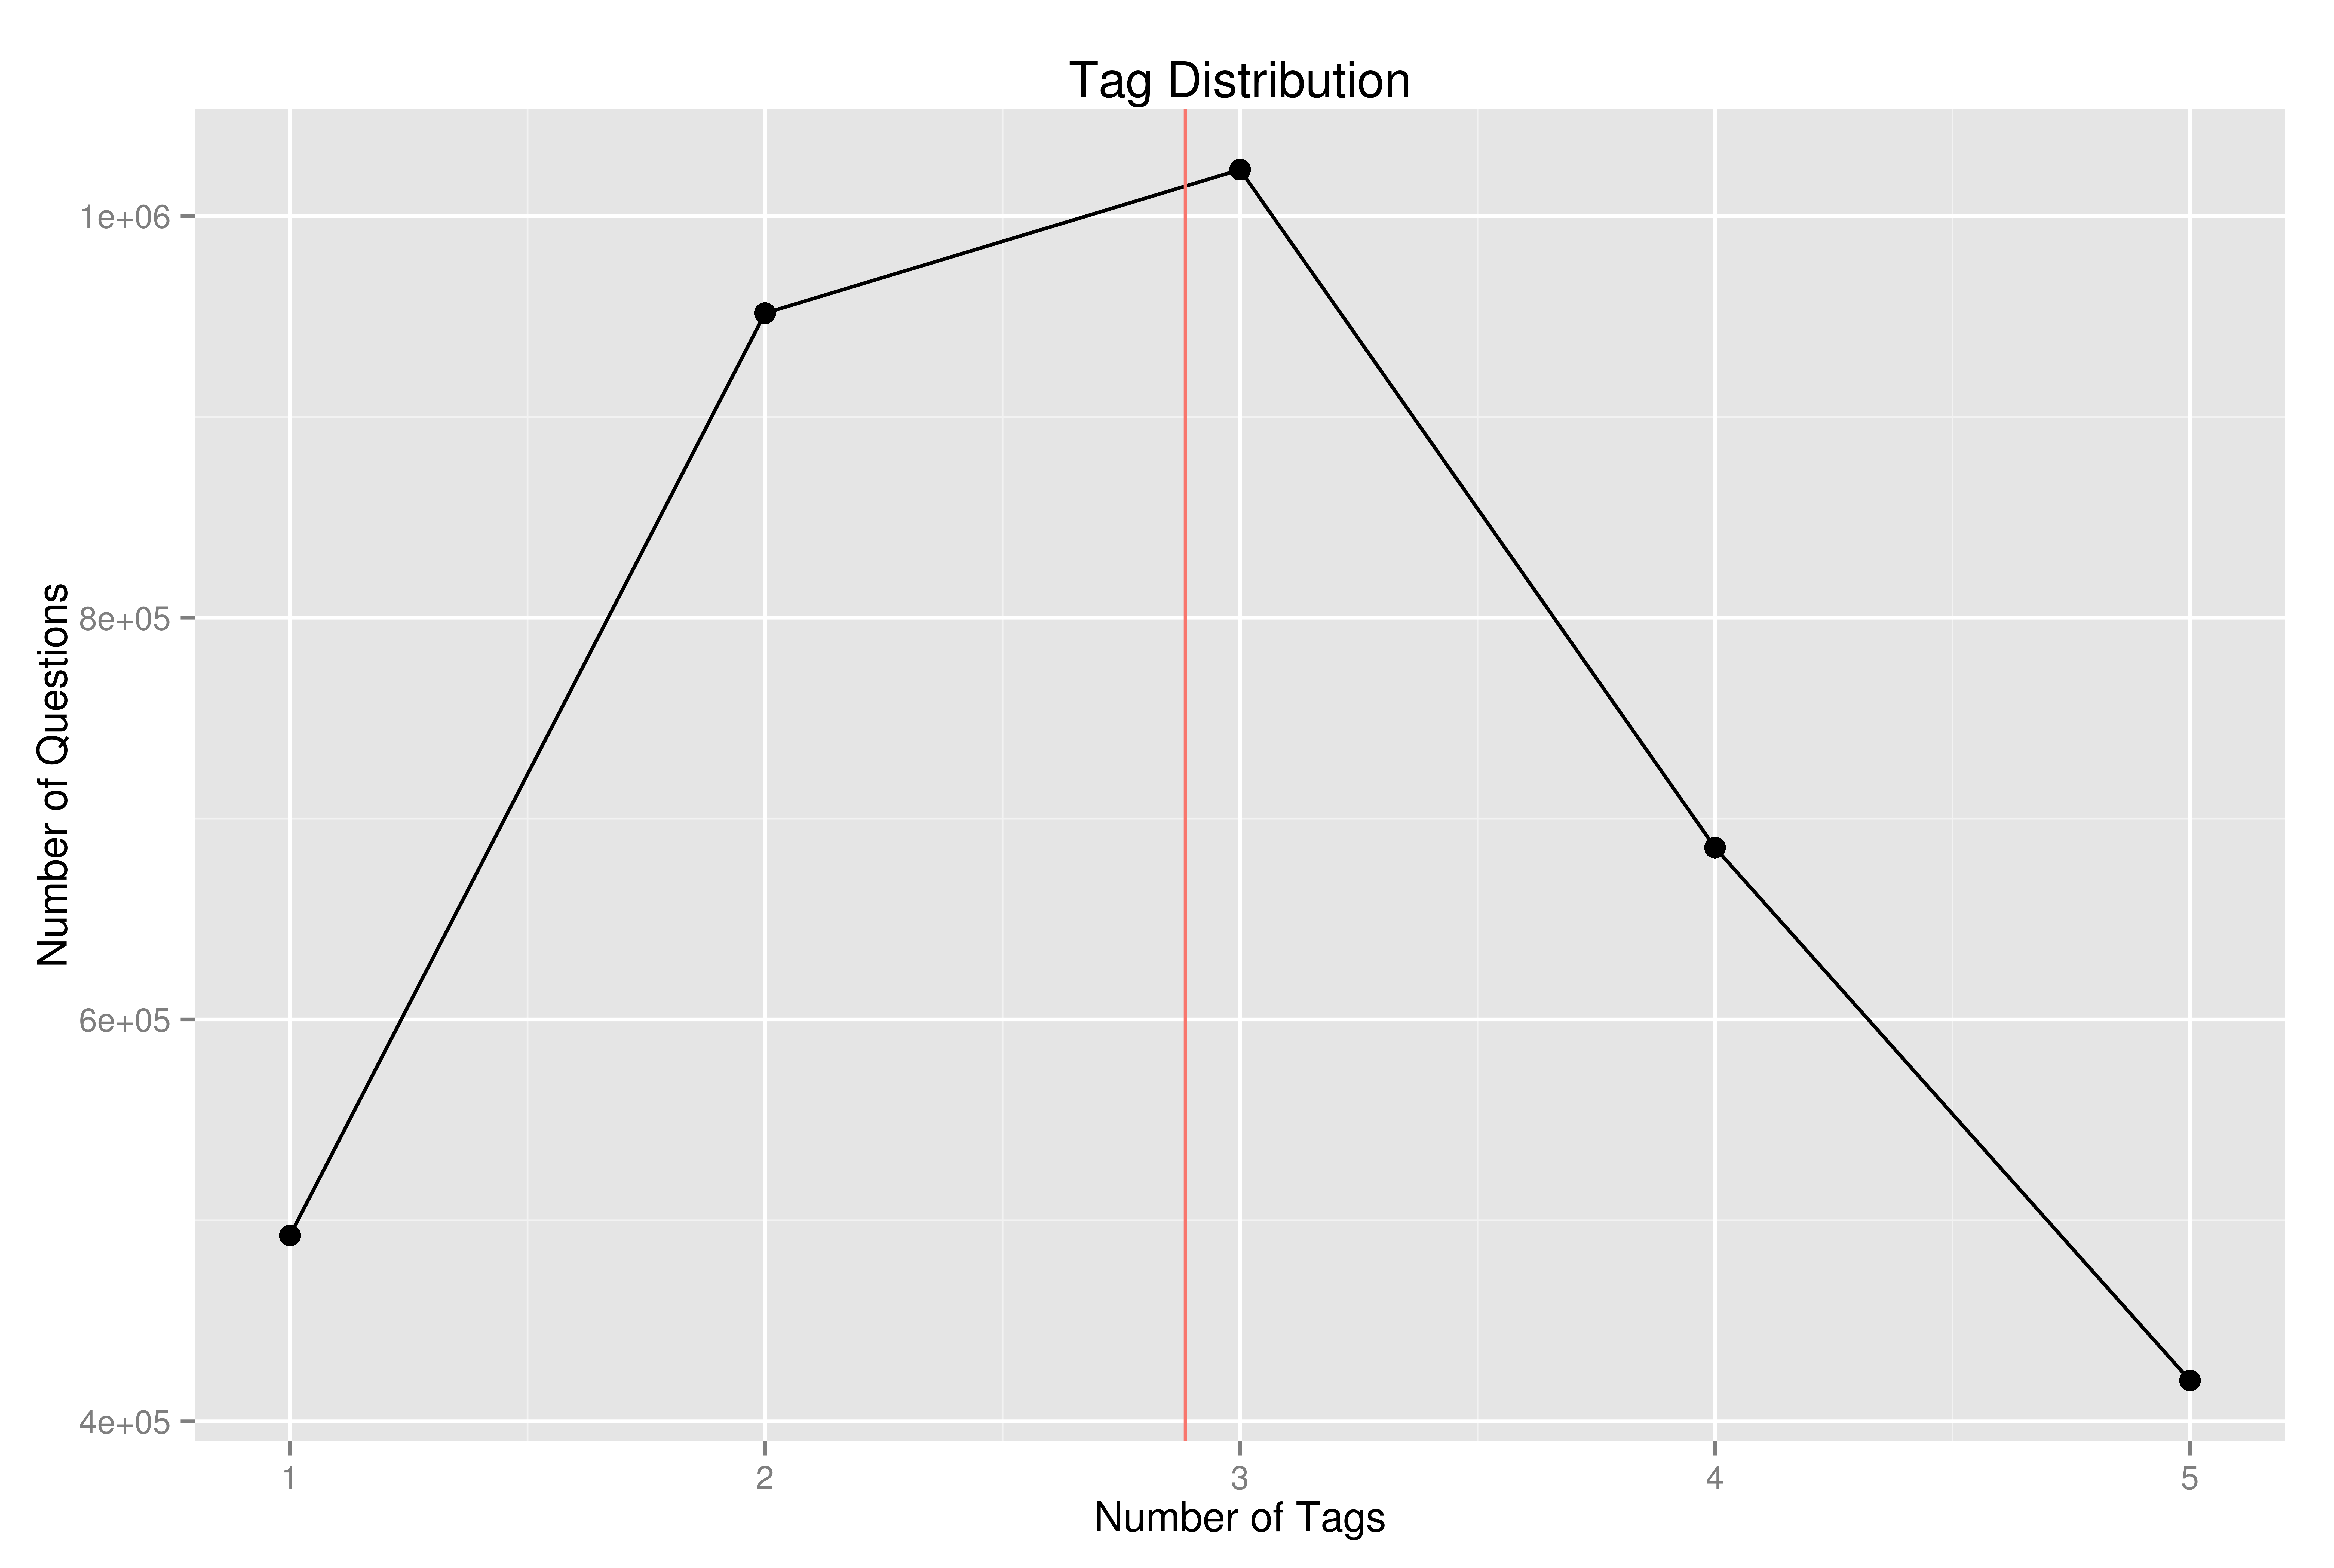
\includegraphics[width=0.5\textwidth]{tag_distribution}
			\label{fig:tag_dist}
			\caption{Distribution of the number of tags per question}
		\end{figure}
	% subsection Data Set Analysis (end)

	\subsection{Outline} % (fold)
	\label{sub:Outline}
		This paper will proceed as follows. Section 2 will cover the technical
		details of our methods including the tools involved, the model
		selection process and a brief description of each model under
		evaluation. Section 3 will show our results of evaluated mean \Fone
		scores for each classifier. Section 4 will interpret our results
		including speculations of why Random Forests perform poorly with Latent
		Semantic Analysis. Finally, Section 5 will conclude with planned future
		work.
	% subsection Outline (end)

% section Introduction (end)

\section{Methods} % (fold)
\label{sec:Methods}
	\subsection{Tools} % (fold)
	\label{sub:Tools}
		The solution is programmed using Python. The implementations of the
		models, cross-validation and metrics are provided in the scikit-learn
		library which is coupled with scikit and numpy.
	% subsection Tools (end)

	\subsection{Problem Decomposition} % (fold)
	\label{sub:Problem Decomposition}
		We begin by decomposing the problem into a set of binary
		classifications tasks: for each tag, generate a classifier that
		predicts whether a given question should have the tag. Each tag must
		therefore have its own training set. We design the training set for
		each tag such that there are exactly $60$ questions with the tag and
		$1500$ questions without the tag. It is then easy to evaluate which
		classifier performs best for a specific tag.
	% subsection Problem Decomposition (end)

	\subsection{Model Selection} % (fold)
	\label{sub:Model Selection}
		In order to select the best model for each tag, several models are
		assessed using cross-validation such that the model with the best mean
		score is used as the classifier for the tag. In particular, we use
		stratified $k$-Fold cross-validation that partitions the training data to
		$k$ folds such that the expected value of the predictions are
		approximately similar across each fold. We select $k$ to be three folds
		since $60$ and $1500$ are equally divisible by three.
	
		Each model assessed uses grid search for hyperparameter optimization.
		That is, the parameters of each model are tuned exhaustively with
		bounds. Once all parameter combinations have been assessed, the
		parameters with the best mean cross-validation score are used in their
		model.
	% subsection Model Selection (end)

	\subsection{Preprocessing} % (fold)
	\label{sub:Preprocessing}
		Since we are using a Bag-of-Words (BOW) approach, we must vectorize the
		data set. That is, for each question, we use a count vectorizer which
		generates a histogram for each of the words in a question. The
		vectorized form is then used as the feature set for training models and
		making predictions.

		A vectorizer's transformation of the data proceeds as follows. First,
		given the corpus of questions, it is tokenized and each token is used
		as a feature. Then, a histogram of the tokens are computed per question
		and stored as rows of a matrix. Hence, this matrix should have dimensions
		$N\times M$ where $N$ is the number of questions and $M$ is the number
		of tokens extracted. We call this matrix, the \emph{question-token
		matrix}. We can visualize this matrix as seen on Figure
		\ref{fig:vectorized_output}.
		\begin{figure}[htbp]
			\centering
			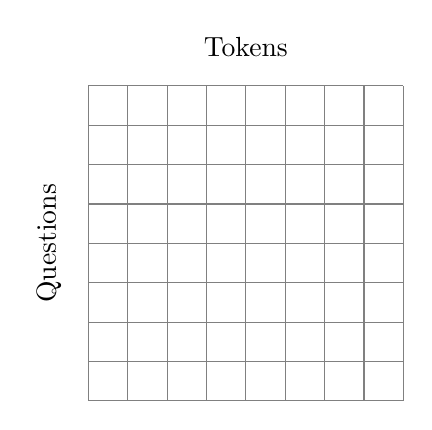
\begin{tikzpicture}
				\draw [step=0.5, gray, thin] (0,0) grid (4,4);
				\node at (2,4.5) {Tokens};
				\node [rotate=90] at (-0.5, 2) {Questions};
			\end{tikzpicture}
			\caption{Question-Token Matrix}
			\label{fig:vectorized_output}
		\end{figure}

		Once the question-token matrix has been computed, an additional
		preprocessing step follows: Latent Semantic Analysis. That is, we apply
		Singular Value Decomposition (SVD) on the matrix to reduce the
		dimensionality. We specify the reduced dimensionality to be $512$ for
		rapid prototyping.
	% subsection Preprocessing (end)

	\subsection{Bernoulli Na\"{i}ve Bayes} % (fold)
	\label{sub:Bernoulli Naive Bayes}
		The na\"{i}ve Bayes approach applies Bayes' theorem in order to
		classify. That is, predicting existence of a tag in a question can be
		reformulated as follows:
		\[
			p(y|\vec{x}) = 
				\frac{p(y) p(\vec{x}|y)}
					{p(\vec{x})}
		\]
		where $y$ is a boolean value representing whether or not the tag should
		exist and $\vec{x}$ is the feature vector of the question. In order to
		compute the classifying value, $y$, we reformulate the problem as an
		optimization problem:
		\[
			\hat{y} = \argmax_y p(y) \prod_{i=1}^{n} p(x_i|y)
		\]
		where the $\hat{y}$ is the classification made.
		
		The Bernoulli variant of na\"{i}ve Bayes assumes that the data is
		distributed according to multivariate Bernoulli distributions. This
		particular implementation is best applied to data sets with a small
		vocabulary (under 1000 features).\cite{mccallum1998} The decision rule
		is based on the following formula:
		\[
				p(x_i|y) = p(i|y)x_i \times (1-p(i|y))(1-x_i)
		\]
		In our solution, we hyperoptimize $\alpha \in \left\{0, 1, 2\right\}$
		which is an additive smoothing parameter.
	% subsection Bernoulli Naive Bayes (end)

	\subsection{Random Forests} % (fold)
	\label{sub:Random Forests}
		The Random Forest approach is an ensemble method that uses a set of weak
		learners to to form a strong learner.\cite{breiman2001} The weak learners are frequently
		decision trees which are grouped together into a forest. The number of
		decision trees generated is parameterized by $T$. Each split of a decision
		tree is computed starting with a random subset of the features of size $m$
		and selecting the best of those features.

		The classification process in Random Forests is as follows. First, the
		feature vector is input into each of the trees of the forest. Then,
		the classification of the classifier should be the class that is the
		voting majority of the trees in the forest.

		In our solution, we hyperoptimize $m \in \left\{\sqrt{N},
		\log_2{N}\right\}$ where $N$ is the number of features and we also
		hyperoptimize $T$.
	% subsection Random Forests (end)

	\subsection{Linear Support Vector Classifier} % (fold)
	\label{sub:Linear Support Vector Classifier}
		The idea of a Support Vector Machine is to define a separating hyperplane
		which distinguishes a set of classes, which, in this case, is a boolean
		value of whether or not a tag should be accepted. There are, however,
		many feasible separating hyperplanes. Hence, we define the optimal
		hyplerplane to be the hyperplane that maximizes the \emph{margin}. The
		margin is defined to be the largest minimum distance of the hyperplane to
		each of the training samples.

		We can compute the optimal hyperplane by reformulating the problem as an
		optimization problem. The primal form of the optimization problem can be
		described as follows:
		\[
			\argmin_{\vec{w}, b} \frac{1}{2}\|\vec{w}\|^2
		\]
		where $\vec{w}$ and $b$ define the optimal hyperplane.

		Since, in our data set, it is rarely the case that the data is linearly
		separable, the optimal hyperplane can be redefined using the \emph{Soft
		Margin} method which 
		\[
			\argmin_{\vec{w}, b, \vec{\xi}} \frac{1}{2}\|\vec{w}\|^2 + C\sum_{i=1}^N \xi_i
		\]
		introduces non-negative slack variables, $\xi_i$, and a penalty
		parameter, $C$.\cite{cortes1995} In our solution, we hyperoptimize $C \in \left\{10^i |
		0 \leq i \leq 9\right\}$ using grid search.
	% subsection Linear Support Vector Classifier (end)

	\subsection{Gradient Boosting Machines} % (fold)
	\label{sub:Gradient Boosting}
		Gradient Boosting Machines (GBM) is an ensemble method on weak
		classifier that builds its model in a stage-wise fashion where each
		stage minimizes a specified loss function using the Gradient Descent
		method.\cite{friedman2001} Each weak classifier is described as a
		function $h(\vec{X};\vec{p}_i)$ where $\vec{X}$ is the input and
		$\vec{p}_i$ is its parameter set. A loss function, $L(\vec{y},
		\vec{y}')$ is then specified on $\vec{y}$ and $\vec{y}'$ which are the
		expected classification and predicted classification respectively. The
		predicted classification is computed as a linear combination of the
		weak learners:
		\[
			\vec{y}' = \sum_{i=1}^K \beta_i h(\vec{X}; \vec{p}_i)
		\]
		where $K$ is the number of weak learners and $\beta_i$ is a weight
		parameter for a specified weak learned, $i$.

		Hence, the model is described by $\vec{\beta}$ and $\vec{P}$ which are the
		weak learner weights and parameter sets respectively. We can then formulate
		the problem as an optimization problem:
		\[
			\argmin_{\vec{\beta}, \vec{P}} L(\vec{y}, \sum_{i=1}^K \beta_i h(\vec{X}; \vec{p}_i))
		\]

		In our solution, we hyperoptimize $K \in \left\{100, 200, 300\right\}$,
		$\text{max\_features} \in \left\{\sqrt{M}, \log_2{M}\right\}$ and
		$\text{min\_samples\_split} \in \left\{1, 2, 3\right\}$.
	% subsection Gradient Boosting (end)
% section Methods (end)

\begin{figure*}[htb!]
	\centering
	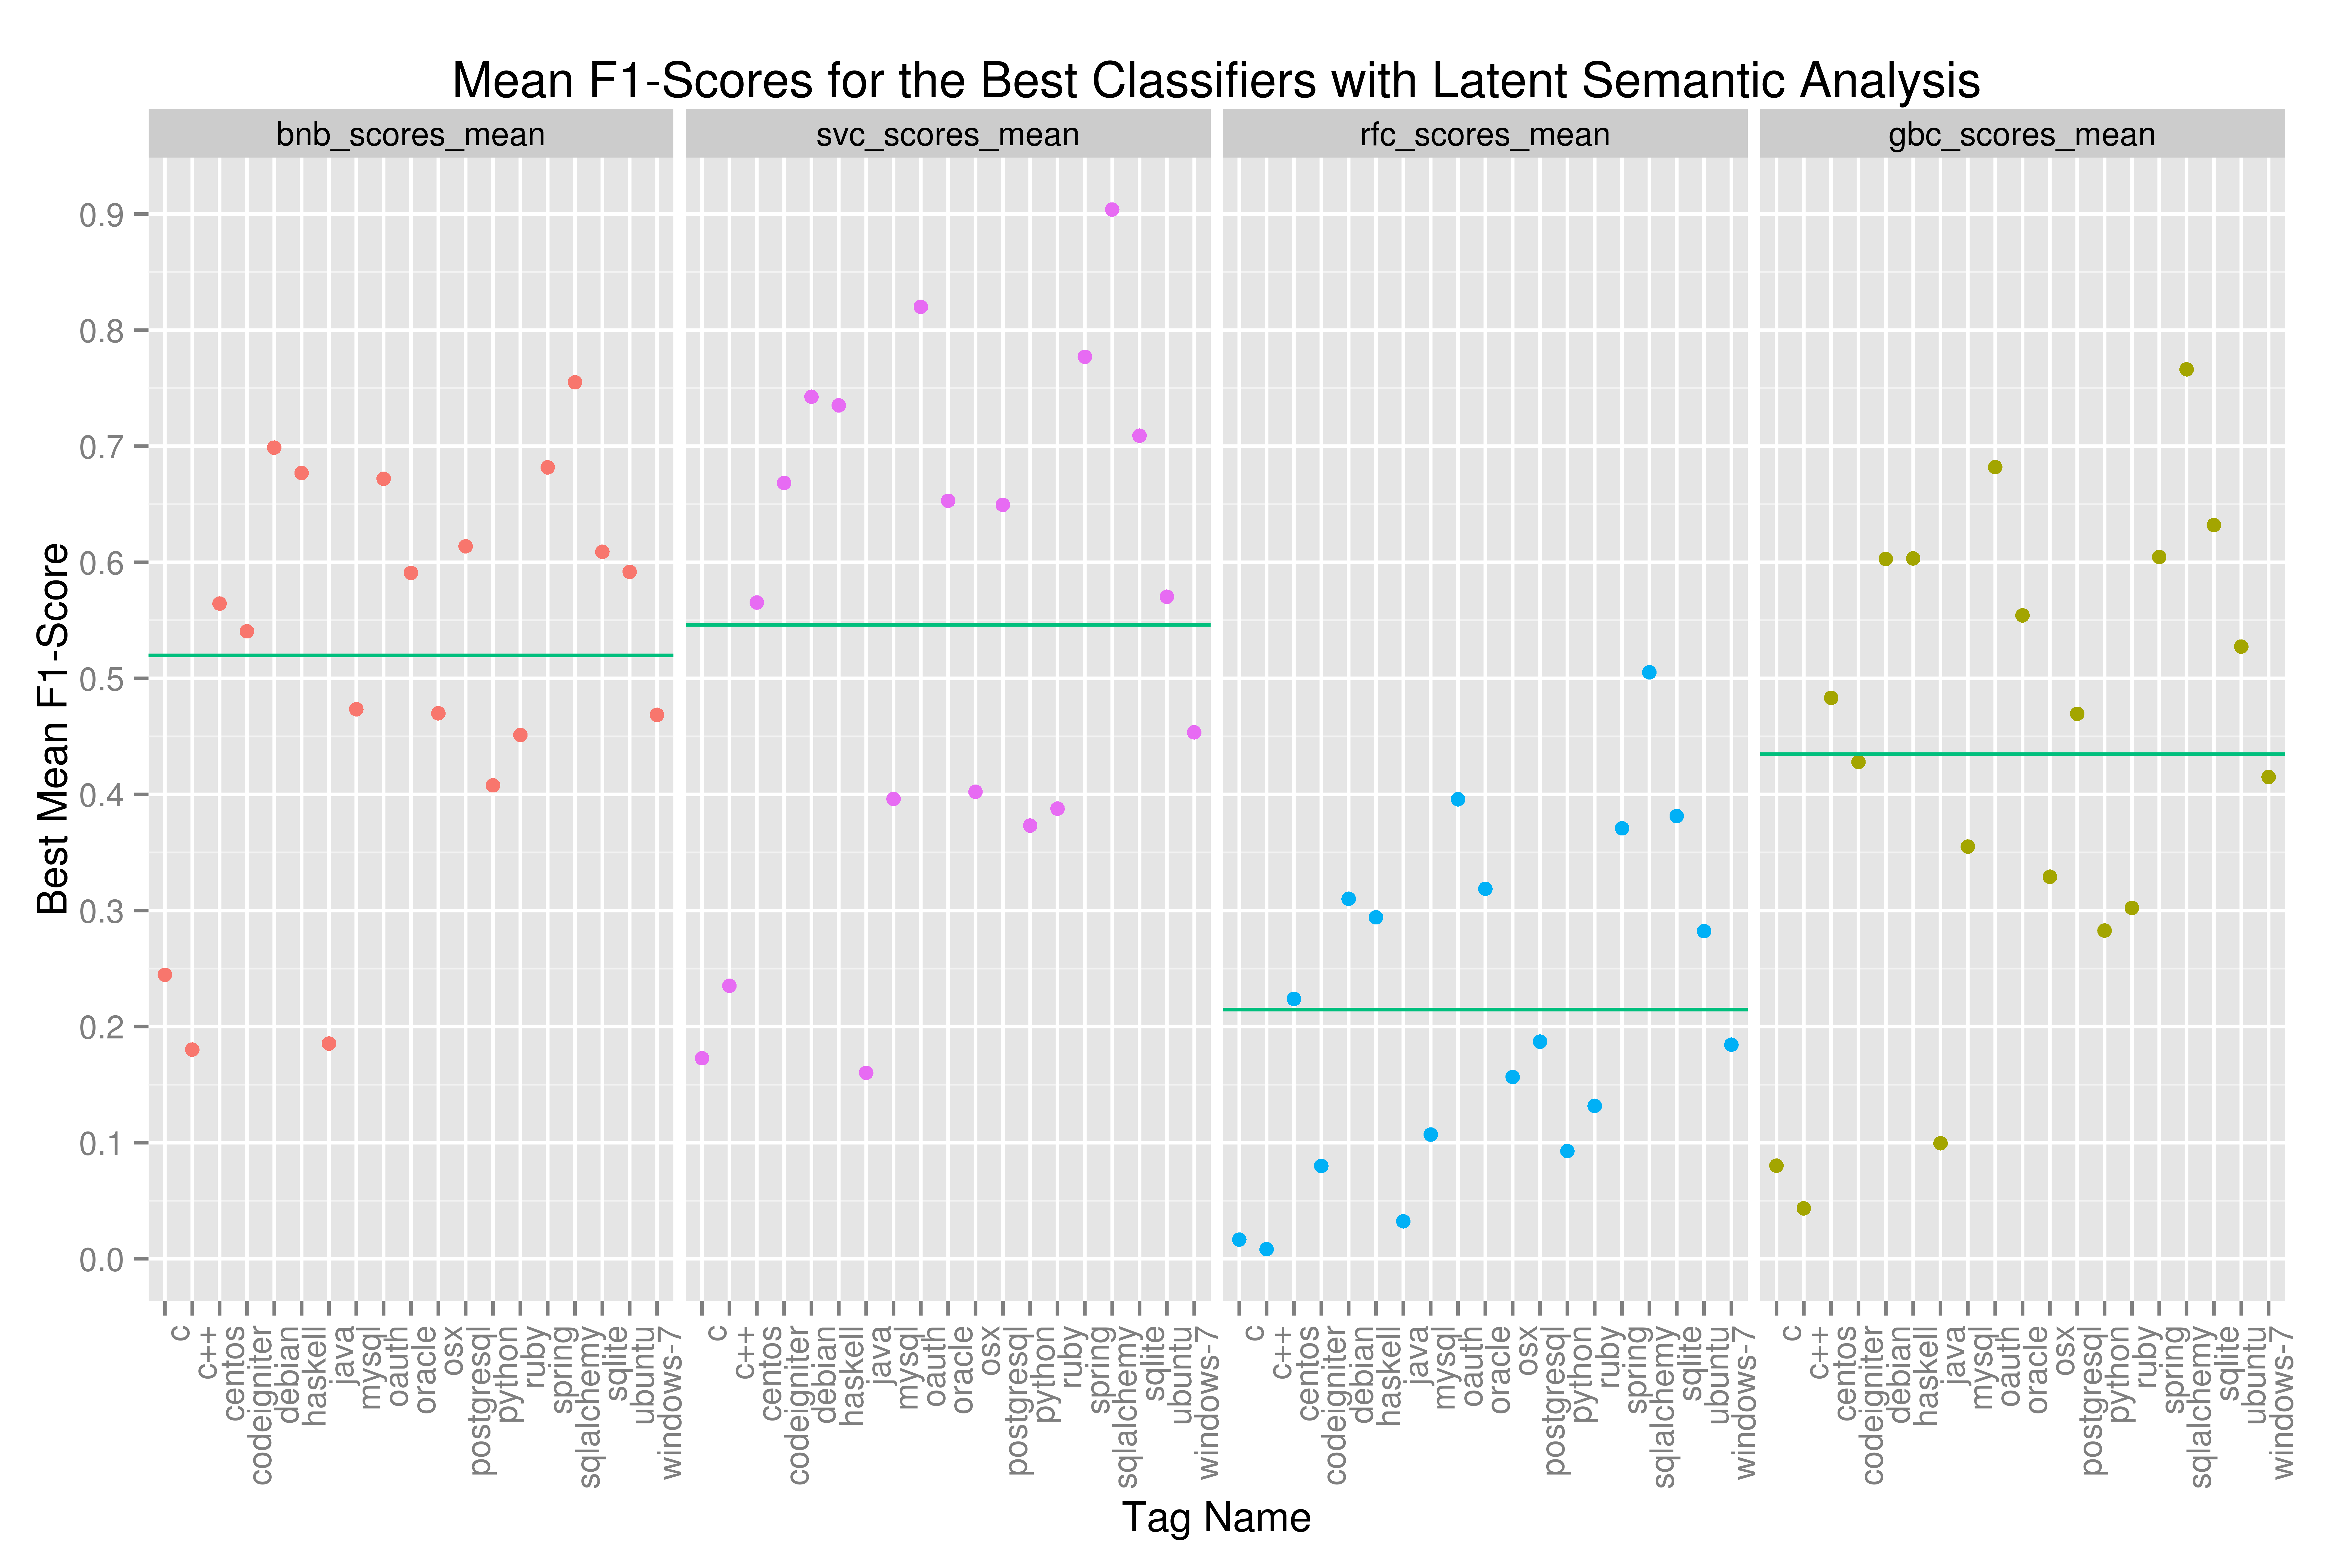
\includegraphics[width=\textwidth]{decomposition}
	\label{fig:decomposition}
	\caption{Mean \Fone-Score decomposition by Classifier}
\end{figure*}

\section{Results} % (fold)
\label{sec:Results}
	The Mean \Fone-Score for the each of the models on the specified subset of
	tags are shown on Table \ref{tab:count_model_scores} and Table
	\ref{tab:lsa_model_scores} which represent scores for models using count
	vectorized features and Latent Semantic Analysis (LSA) respectively. With
	LSA, Bernoulli na\"{i}ve Bayes and Gradient Boosting Machines perform
	significantly better; however, Random Forests perform significantly worse.
	The loss of accuracy in SVMs with LSA is negligible. Generally, SVMs yield
	the best results in both feature sets; however, with LSA, the na\"{i}ve
	Bayes approach sometimes generates a better classifier. A graph of the
	results of classifier scores using LSA is shown in Figure
	\ref{fig:decomposition}.

	We can rank classifiers according to their mean \Fone-score as seen in
	Figure \ref{fig:decomposition}. In order, the best classifiers are SVMs,
	Bernoulli na\"{i}ve bayes, Gradient Boosting Machines and Random Forests in
	that order.
% section Results (end)

\section{Discussion} % (fold)
\label{sec:Discussion}
	Overall, the classifiers had the best accuracy for specific and uncommon tags
	such as "sqlalchemy." Conversely, the classifiers had the worst accuracy for
	popular tags such as "c", "c++" and "python". It is interesting to note that
	"haskell" was accurately classified often. We believe that that popular tags
	are hard to classify because they can easily be associated with unrelated
	terms; in other words, there is a significant amount of noise associated
	with popular tags.

	We believe that the data has a significant amount of high-dimensional noise
	which can be observed through the poor scores of nonlinear classifiers.
	That is, it may be the case that the nonlinear classifiers are overfitting
	due to the significant variance in the methods. The explained variance also
	supports our hypothesis that popular tags are polluted with noisy features.
	Therefore, on the next training phases, it is logical to hyperoptimize over
	parameters that reduce variance in the classifiers.

	The introduction of Latent Semantic Analysis (LSA) made a significant
	impact on the majority of the classifiers. We suspect the loss of accuracy
	in Random Forests using LSA is due to the fact that Random Forests already
	performs a type of dimensionality reduction in its weak learners by
	randomly selecting subsets of the designated feature set. Hence, reducing
	dimensionality with LSA before fitting Random Forests yields redundant
	dimensionality reduction
% section Discussion (end)

\section{Conclusion} % (fold)
\label{sec:Conclusion}
	Although the overall accuracy is low, we have established a baseline metric
	for evaluating further methods to be used in this competition. There is
	much future work to be done such as using Parts-of-Speech as a feature set
	which Latent Semantic Analysis does not take into consideration. Another
	potential feature for programming languages in specific is to design
	specific language classifiers using the known publicly available syntax and
	grammar specifications of each language.

	In order to solve the bias-variance dilemma, we may consider an ensemble
	method which produces a classification based on bagging or boosting the
	given models. The running time of learning strong models may, however, be a
	concern. Furthermore, Stochastic Gradient Descent Boosting is a natural
	consideration to tackle the issue of variance.
% section Conclusion (end)

\section{Acknowledgements} % (fold)
\label{sec:Acknowledgements}

We would like to thank the Stack Exchange communities for making available
their data set.

% section Acknowledgements (end)

\bibliographystyle{plain}
\bibliography{so_tagging}

\begin{table*}[ht!]
	\centering
	\begin{tabular}{|l|c|c|c|c|}
		\hline
		\textbf{Tag} & \textbf{Bernoulli Na\"{i}ve Bayes} & \textbf{Linear Support Vector Classifier} & \textbf{Random Forests} & \textbf{Gradient Boosting} \\\hline
		codeigniter	& 0.1764	& 0.7202	& 0.5176	& 0.6122 \\\hline
		spring		& 0.2957	& 0.7268	& 0.4874	& 0.6456 \\\hline
		sqlalchemy	& 0.3516	& 0.8959	& 0.7742	& 0.8543 \\\hline
		oauth		& 0.4117	& 0.8238	& 0.4157	& 0.6899 \\\hline
		mysql		& 0.1256	& 0.3877	& 0.0240	& 0.2006 \\\hline
		oracle		& 0.1817	& 0.6398	& 0.2893	& 0.5034 \\\hline
		postgresql	& 0.1957	& 0.6299	& 0.5194	& 0.3807 \\\hline
		sqlite		& 0.1731	& 0.7293	& 0.4919	& 0.5642 \\\hline
		ubuntu		& 0.2694	& 0.5701	& 0.2040	& 0.4390 \\\hline
		debian		& 0.3079	& 0.7239	& 0.5674	& 0.7042 \\\hline
		centos		& 0.2353	& 0.5878	& 0.1641	& 0.3173 \\\hline
		osx			& 0.1283	& 0.4061	& 0.1635	& 0.3469 \\\hline
		windows-7	& 0.2498	& 0.4527	& 0.0465	& 0.2070 \\\hline
		python		& 0.0921	& 0.3181	& 0.0951	& 0.1563 \\\hline
		java		& 0.0727	& 0.1725	& 0.0081	& 0.0662 \\\hline
		c++			& 0.1291	& 0.2110	& 0.0082	& 0.0830 \\\hline
		c			& 0.1314	& 0.2962	& 0.0313	& 0.1168 \\\hline
		ruby		& 0.0978	& 0.3972	& 0.1328	& 0.2048 \\\hline
		haskell		& 0.2524	& 0.7708	& 0.7378	& 0.6077 \\\hline
	\end{tabular}
	\caption{Mean $F_1$-Scores of Models with Count Vectorized Feature Vectors}
	\label{tab:count_model_scores}
\end{table*}

\begin{table*}[ht!]
	\centering
	\begin{tabular}{|l|c|c|c|c|}
		\hline
		\textbf{Tag} & \textbf{Bernoulli Na\"{i}ve Bayes} & \textbf{Linear Support Vector Classifier} & \textbf{Random Forests} & \textbf{Gradient Boosting} \\\hline
		codeigniter	& 0.5405	& 0.6683	& 0.0799	& 0.4278 \\\hline
		spring		& 0.6817	& 0.7770	& 0.3708	& 0.6045 \\\hline
		sqlalchemy	& 0.7551	& 0.9038	& 0.5051	& 0.7662 \\\hline
		oauth		& 0.6719	& 0.8200	& 0.3958	& 0.6820 \\\hline
		mysql		& 0.4733	& 0.3961	& 0.1069	& 0.3550 \\\hline
		oracle		& 0.5908	& 0.6530	& 0.3187	& 0.5542 \\\hline
		postgresql	& 0.6137	& 0.6495	& 0.1870	& 0.4694 \\\hline
		sqlite		& 0.6090	& 0.7090	& 0.3813	& 0.6321 \\\hline
		ubuntu		& 0.5917	& 0.5702	& 0.2821	& 0.5273 \\\hline
		debian		& 0.6987	& 0.7426	& 0.3100	& 0.6028 \\\hline
		centos		& 0.5644	& 0.5653	& 0.2238	& 0.4831 \\\hline
		osx			& 0.4699	& 0.4023	& 0.1565	& 0.3290 \\\hline
		windows-7	& 0.4685	& 0.4535	& 0.1844	& 0.4149 \\\hline
		python		& 0.4078	& 0.3731	& 0.0927	& 0.2826 \\\hline
		java		& 0.1853	& 0.1601	& 0.0322	& 0.0995 \\\hline
		c++			& 0.1801	& 0.2352	& 0.0082	& 0.0434 \\\hline
		c			& 0.2446	& 0.1727	& 0.0164	& 0.0801 \\\hline
		ruby		& 0.4512	& 0.3877	& 0.1316	& 0.3022 \\\hline
		haskell		& 0.6769	& 0.7351	& 0.2941	& 0.6033 \\\hline
	\end{tabular}
	\caption{Mean $F_1$-Scores of Models with Latent Semantic Analysis}
	\label{tab:lsa_model_scores}
\end{table*}

\end{document}
